\documentclass[a4paper,10pt]{report}

\usepackage[utf8]{inputenc}
\usepackage{ulem}
\usepackage[frenchb]{babel}
\usepackage{graphicx}
\usepackage[final]{pdfpages}
\usepackage{url}
\usepackage{xcolor}
\usepackage{listings}
\lstset{language=java, frame=single, breaklines=true, frameround=fttt,
captionpos=b}

\begin{document}
\author{Jerome NAHELOU, Quentin NEBOUT, Romain SOLVE, Fabien QUINTARD}


\chapter[Implémentation]{Implémentation} 
\section{L'objet Caméra}
\subsection{Description}
L'objet Camera est implémenté dans la classe \textit{Camera.java}. \\
Celle-ci y regroupe les informations suivante : 
\begin{itemize} 
\item un descriptif de la caméra. Exemple : ``Caméra du Jardin''
\item le protocole de communication à utiliser (http ou rtsp).
\item l'url d'acces. Exemple : ``http://192.168.1.20''
\item le port (par defaut le port 80 est utilisé).
\item le nom d'utilisateur (login).
\item le mot de pass.
\item le canal (necesaire lors de l'utilisation de plusieurs caméras pour une
meme adresse).
\item un identifiant unique appelé \textit{uniqueID} definit par la position de
la caméra dans la liste sur la page d'acceuil.
\item le groupe assigné lors de la mise en route de la détéction de mouvement
(compris entre 0 et 9) appelé \textit{groupeID}.\\
\end{itemize}
Afin de pouvoir communiquer une caméra entre plusieurs \textit{activitées
(activity)} nous avons choisi de rendre cette classe \textit{serializable} pour
ne pas devoir passer une a une chaques caracteristiques.\\
Cette classe contient également une primitive capable de générer un entier
unique pour le couple \textit{uniqueID} et \textit{groupID} afin de pouvoir
lancer plusieurs fenetres de detection de mouvement pour une meme caméra
(\textit{getMotionDetectionID}).

\subsection{Construction de l'objet}
La création d'une caméra se fait via l'interface graphique definit par le
fichier \textit{add\_cam.xml}.\\
\begin{center}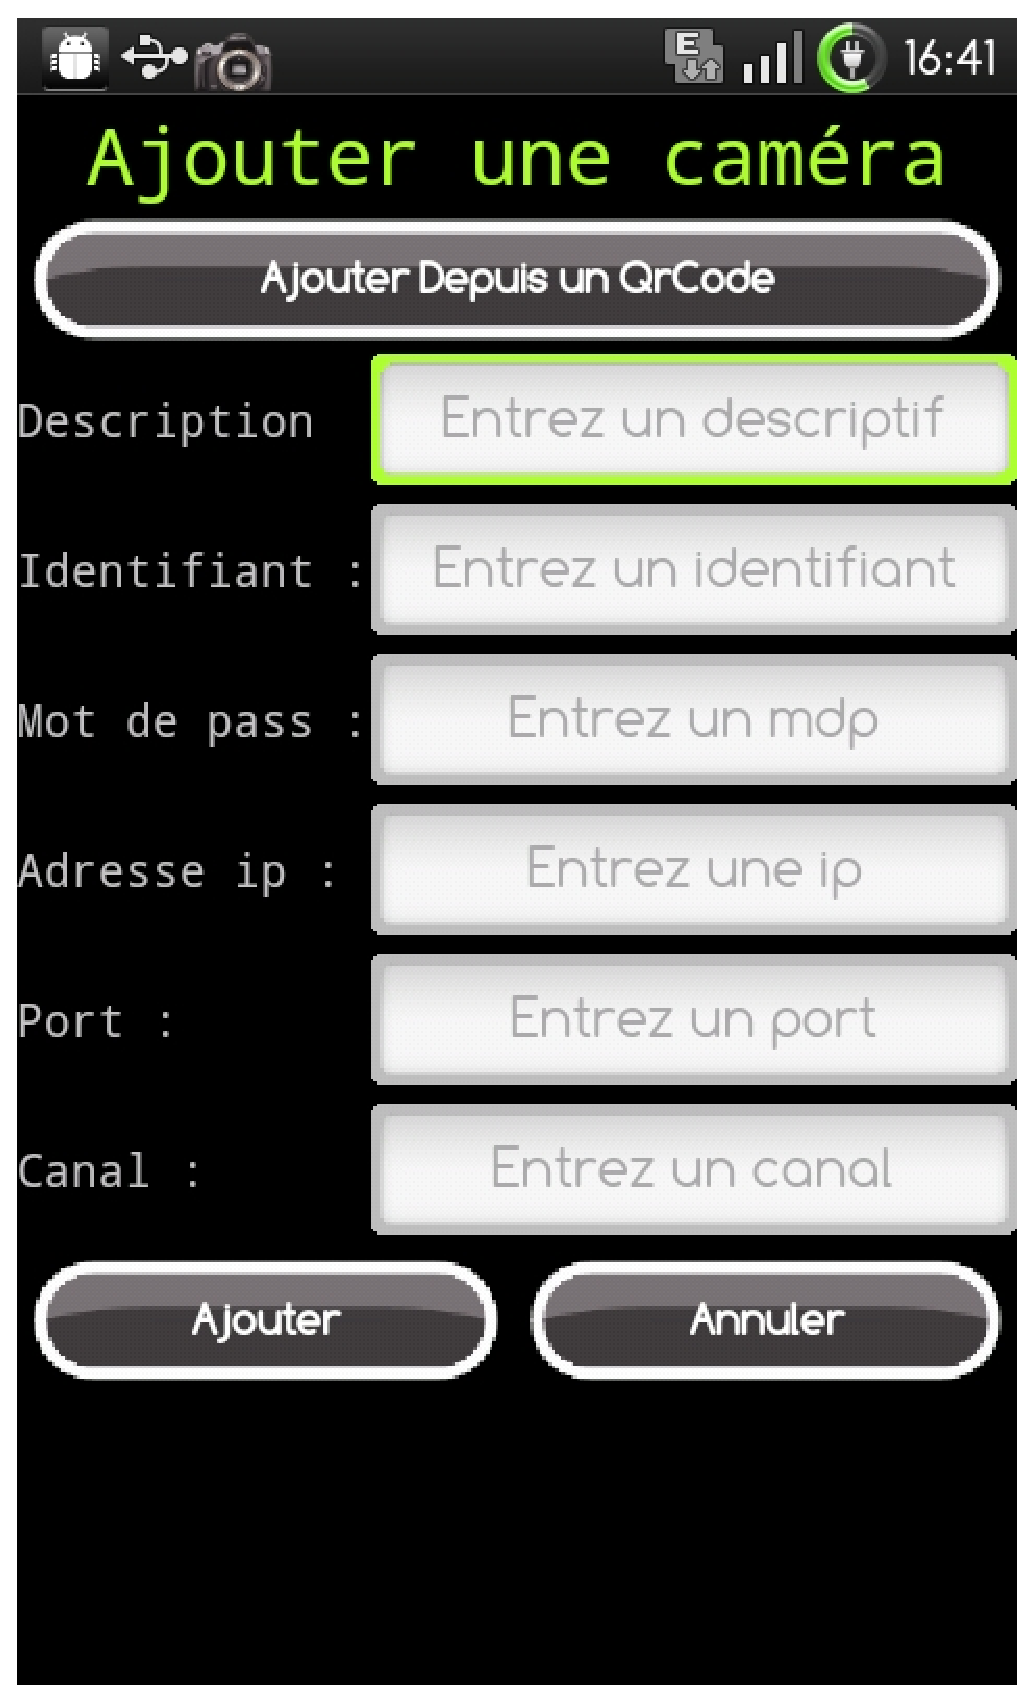
\includegraphics[scale=0.5]{Images/addCamScreenShot.eps} \newline
\end{center} 
On y retrouve des champs de texte édiatable pour chacunes des caracteristiques
de la caméra ainsi qu'un bouton permettant l'ajout de caméra via
\textit{QrCode}.
\indent Le lecteur de code Qr est implémenté par la bibliothèque
\textit{zxing} \footnote{\label{zxing} http://code.google.com/p/zxing/}. \newline
Lors d'un clic sur ce bouton, nous appelons l'activité 
\textit{SCAN} de la bibliotheque zxing avec comme argument
\textit{QR\_CODE\_MODE}.\\
Si la bibliothèque n'est pas disponible sur l'appareil, nous faisons appel a
\textit{l'android market} afin de telecharger l'application \textit{zxing} (qui
implémente l'ensemble des fonctions proposées par la bibliothèque).
\newpage
\begin{lstlisting}[caption={Lancement de l'activité zxing ou de l'android
market}] 
    public void onClick(View v) { try {
            Intent intent = new Intent(
                "com.google.zxing.client.android.SCAN");
            intent.putExtra("SCAN_MODE", "QR_CODE_MODE");
            startActivityForResult(intent, 0);
        } catch (ActivityNotFoundException e) {
            String marketSearch = "market://details?id=com.google.zxing.client.android";
            Intent updateIntent = new Intent(Intent.ACTION_VIEW, Uri.parse(marketSearch));
            startActivity(updateIntent);
        }
    }
\end{lstlisting}
\indent Lorsque l'activitée \textit{zxing} se termine, l'activité
\textit{addCam} recupere l'adresse de la caméra contenu dans le code Qr puis verrouille les
champs de texte édiatable adresse et port.\\
\indent Pour ajouter la nouvelle
caméra, il ne reste plus à l'utilisateur qu'à cliquer sur le bouton \textit{ajouter} pour revenir sur l'écran d'acceuil et constater
l'ajout de la caméra. Cependant il reste possible de revenir à l'écran d'acceuil
sans sauvegarder les changement en cliquant sur \textit{fermer}.

\subsection{Affichage des Caméras}


\subsection{Modification de l'objet}



\end{document}
